\documentclass{amsart}
\usepackage{amsmath}
\usepackage{amssymb}
\usepackage{amsthm}
\usepackage{listings}
\usepackage{geometry}
\usepackage{float}
\usepackage{mathtools}
\DeclarePairedDelimiter{\ceil}{\lceil}{\rceil}
\usepackage{graphicx}
\geometry{a4paper}

\newtheorem{thm}{Theorem}
\newtheorem{prop}{Proposition}
\newtheorem{lem}{Lemma}
\newtheorem{cor}{Corollary}
\newtheorem{rem}{Remark}
\newtheorem{exa}{Example}
\newtheorem{clm}{Claim}

\theoremstyle{definition}
\newtheorem{definition}{Definition}[section]

\newtheoremstyle{case}{}{}{}{}{}{:}{ }{}
\theoremstyle{case}
\newtheorem{case}{Case}

\title{Prime Generation Draft}
\author{Jason Medcoff}
\date{November 15, 2017}

\begin{document}
    \maketitle
    
    \begin{abstract}
    	The generation of large primes has been of great importance to modern cryptography. In this paper we review a widely known and deceptively efficient method for generating prime numbers: the Sieve of Eratosthenes. We build up to the algorithm with a review of some basic properties of primes and composites, and develop some results that make the sieve more efficient in practice.
    	Emphasis is placed on the mathematics behind the algorithm, with the intention of educating the student of computer science student about the significance of its time complexity.
    \end{abstract}
    
    % Outline
    % Intro: Review of some properties of primes
    %        fundamental theorem of arith
    %        factors less than the square root
    %        
    % Body:  The Sieve of Eratosthenes
    %        proof of the algo: correctness, time complexity
    %        code, examples
    %        Potential Improvement
    %        wheel factorization? (maybe)
    % Segmented sieve and/or sieve of Sundaram
    %
    % Conclusion
    
    
    \section{Introduction}
    
    Today, the generation of prime numbers is a task generally associated with hashing algorithms, public key cryptography, and searching for factors of large numbers. Most modern algorithms designed to generate primes are derived from a process devised by Eratosthenes of Cyrene in Ancient Greece. In this paper, we explore the motivating ideas about prime numbers that lead to the intuitive derivation of the Sieve of Eratosthenes, beginning with some review of elementary number theory concerning primes and composites.
        
    The algorithm is decidedly easy to understand, and similarly easy to implement in one's favorite programming language. In fact, the careful eye may notice potential areas of improvement in the interest of time and space. It is perhaps not surprising, then, that most modern prime generation algorithms are derived from the fundamental prime sieve due to Eratosthenes.
    
    We begin by reviewing the essential ideas of primes and composites. The Fundamental Theorem of Arithmetic describes that all numbers have a factorization of primes only, unique up to the ordering of the factors. In addition, it can be shown that at least one of a number $n$'s factors must lie in the range $[2, \sqrt{n}]$. Combining these results, we can show that for any number $n$, a prime factor in this range implies that $n$ is composite. From this, it is easily seen that to generate the primes up to $n$, we need only cross out the multiples of numbers less than $\sqrt{n}$.
    
    Following this important result, we have all we need to implement a simple version of the Sieve of Eratosthenes, at six lines of code. It is shown by proof of correctness that the algorithm produces all primes up to $n$. By applying Mertens's Second Theorem, we can derive the sieve's asymptotic running time. Next, a time test is performed, demonstrating the running time in practice, and we see that the asymptotic running time bounds the experimental trials.
    
    Next, we observe areas of potential improvement of the algorithm, verify the ideas for improvement, and modify the algorithm. 
    
    
    \section{Some Basics of Primes and Composites}
    
%    By the Fundamental Theorem of Arithmetic, the prime numbers are demonstrated to be the key ingredients to producing the set of integers. Despite their significance, we know very little about where to find primes within the integers. Perhaps the biggest unsolved problem in mathematics today, the Riemann Hypothesis, makes a suggestion about the asymptotic distribution of the primes.
	
	Understanding of the prime number sieve depends upon an understanding of some important properties of prime numbers. The ideas of checking up to the square root of a number for factors and unique factorizations of composites are developed in this section. We begin with familiar definitions, and then move into groundwork that will allow the correctness of the sieve to be shown.

	Recall the following definition.
	\begin{definition}
		A natural number $p>1$ is said to be prime if its only positive divisors are 1 and $p$. If $p$ is not prime, it is said to be composite.
	\end{definition}
	
	One of the most important theorems with regards to the primes and integers follows.
	\begin{thm}[Fundamental Theorem of Arithmetic]\label{arith}
		If $n > 1$ is a natural number, it can be written as a product of powers of primes unique up to the order of the factors.
	\end{thm}
	\begin{proof}
		Suppose there exists an integer $n>1$ such that $n$ cannot be written as a product of primes. By the well-ordering principle, we know that there must be a smallest $n$ satisfying this. Write $n$ as a product, $n = xy$, with $x>1$ and $y<n$. Since $n$ is the smallest positive integer that cannot be written as a product of primes, and $x$ and $y$ must be less than $n$, we can write $x$ and $y$ as products of prime factors. Then $n$ can be written as a product of primes, which contradicts the above assumption. So, every integer $n>1$ can be written as a product of primes.
		
		Next, suppose an integer $n>1$ has two prime factorizations, such that
		$$ n = j_1 \cdots j_s = k_1 \cdots k_t $$
		where all $j_i$ and $k_i$ are prime. By the well-ordering principle, we know that there must be a smallest $n$ satisfying this as well. Then $j_1 | n = k_1 \cdots k_t$ and since $j_1$ is prime, it must divide $k_i$ for some $i$. But we know that $k_i$ is prime too, so it must be that $j_1 = k_i$. Then we relabel $k_i$ as $k_1$ for simplicity, and we now cancel $j_1$ to obtain
		$$ j_2 \cdots j_s = k_2 \cdots k_t . $$
		Since $n$ is the smallest positive integer that has a non-unique prime factorization, and $ j_2 \cdots j_s = k_2 \cdots k_t < n $ is a product of primes, we arrive at a contradiction. Then there cannot exist an integer $n>1$ with two different factorizations.
	\end{proof}

	An immediate question resulting from this theorem is how we can best obtain the prime factors of arbitrary numbers. This question is still open in number theory and theoretical computer science; no classical algorithm is known that can factor a number in polynomial time on the number of digits. The difficulty of factoring very large numbers (on the order of thousands of digits) led to the creation of the RSA cryptosystem.
	
	Given some number $n$, we may want to find out whether $n$ is prime or composite. Naively, we can simply enumerate the natural numbers starting at 2, and check for divisibility, stopping when we reach $n$. However, in the interest of saving time, we can apply a result that will cut down the time spent checking divisors.
	\begin{lem}\label{sqrt}
		If $n$ is composite, at least one of its factors lies in $[2, \sqrt{n}]$.
	\end{lem}
	\begin{proof}
		Let $m = \sqrt{n}$. Then we can write $n$ as
		$$ n = m \cdot m = a \cdot b . $$
		Consider $a$. One of the following must be true: $a>m$, $a<m$, or $a=m$. In the first case, $b$ must be less than $m$; in the second case, $b$ will be greater than $m$. If $a=m$, clearly $b=m$. Therefore, if we search the integers up to $m$, we will find at least one factor of $n$.
	\end{proof}
	
	We can combine this result with the fundamental theorem of arithmetic, and easily show the following.
	\begin{cor}\label{corprime}
		Let $n>1$ be an integer. If $n$ does not have a prime factor in the range $[2, \sqrt{n}]$, it is prime.
	\end{cor}
	This is a combination of the contrapositive of lemma \ref{sqrt} with theorem \ref{arith}. So now, we have a way to check for primality of small numbers. For some $n$, we need only check divisibility by primes in $[2, \sqrt{n}]$. This algorithm, called trial division, is shown to be very slow on larger numbers.
	
	\begin{figure}[H]\caption{Trial Division}
		\begin{lstlisting}[language=Python]
		def trialdivision(n):
		    composites = set()
		    for i in range(4, n):
		        for j in range(2, i):
		            if i % j == 0:
		                composites.add(i)
		return [x for x in range(2,n) if x not in composites]
		\end{lstlisting}
	\end{figure}
	
	This implementation begins at 4 and iterates up to $n$. Each number is checked for factors. If a factor is not found up to the number, we leave it be. If a number is found to be composite, it is ``marked" by collecting it into a set. When the algorithm outputs at the end, it iterates through the numbers up to $n$ and gives those numbers that were not marked as composite.
	
	% TODO: Prove asymptotic time complexity of trial division
	
	\begin{thm}
		The trial division algorithm has an asymptotic running time of $O(n^2)$.
	\end{thm}
	\begin{proof}
		Consider the set update operations: we will count the number of times we update the \texttt{composites} set. The outer loop iterates $n-1$ times, and the inner loop iterates $i-1$ times. We can write the number of times \texttt{composites.add} is called as
		\begin{equation*}
		\begin{split}
		\sum_{i=2}^{n} \sum_{j=2}^{i} 1 & = \sum_{i=2}^{n} i-2+1 \\
		& = \sum_{i=2}^{n} (i-1) \\
		& = \frac{n(n+1)}{2} - 1 - (n-1) \\
		& = \frac{n^2 - n}{2} \\
		& = O(n^2)
		\end{split}
		\end{equation*}
	\end{proof}
	
	So while trial division is the most naive way to generate primes, it is far from the most efficient. Note that we can also use trial division to check some particular number for primality. This is also inefficient for large numbers.
	
	
	\section{Generating Primes with the Sieve of Eratosthenes}
	
	The Sieve of Eratosthenes is a process for generating primes up to some positive integer $n$. Roughly speaking, the process is to cross off the multiples of the numbers up to the square root of $n$. Those numbers that remain are the primes up to $n$. Here we outline who Eratosthenes was, and then discuss his algorithm. The correctness of the process is rigorously argued, and then the time complexity is derived. A timed experiment is then performed to show the running time in practice.
	
	\subsection{Eratosthenes of Cyrene}	
	Eratosthenes was born in Ancient Greece, in 276 BCE. He was a scholar, and had a career as the librarian at Alexandria. During his life, he made many contributions to geography; he provided accurate maps of the world, and made some of the most realistic estimates of land area of the time. He also studied climate zones, and made predictions about temperature differences of the world. 
	
	Perhaps his most well known achievement was measuring the circumference of the earth to a surprising degree of accuracy. Eratosthenes first assumed that rays from the sun traveled to the earth in parallel paths. He measured the noon shadow at Alexandria to be 7.2 degrees in angle. At this time, he believed the sun to be directly overhead at Syrene, Egypt. Using the distance from Syrene to Alexandria, he calculated the circumference to be 23300 miles, with an error of only about 1500 miles. 
	
	\subsection{The First Sieve Algorithm}
	
	During his time as a librarian, Eratosthenes developed an efficient method for generating prime numbers. He began by listing integers up to some bound. After crossing off the multiples of every number below the square root of the upper bound, every number remaining would be prime.
	
	Consider the following algorithm.
	
	\begin{figure}[H]\caption{Sieve of Eratosthenes}
		\begin{lstlisting}[language=Python]
		def Eratosthenes(n):
		    primes = []
		    composites = set()
		    for i in range(2, n+1):
		        if i not in composites:
		            primes.add[i]
		            composites.update(range(i**2, n+1, i))
		    return primes
		\end{lstlisting}
	\end{figure}
	
	The python code above utilizes the ``set" data structure; this is suitable for two reasons. First, since we are only considering one list of numbers 2 to $n$, every element we are considering is unique, suggesting the use of a set. Second, the code performs many membership checks. For lists, checking membership in a list of length $m$ is $O(m)$ in the average case, while for sets this check is $O(1)$, or constant time, regardless of the set's size.
	
	\begin{thm}
		The algorithm \texttt{Eratosthenes} produces the prime numbers in the range $[2, n]$.
	\end{thm}
	\begin{proof}
		The algorithm's correctness is easy to see based on the use of \texttt{composites}. The loop invariant here is that the set \texttt{composites} contains all composite numbers between 2 and $i$; this holds for every iteration, where we yield $i$ if it is not composite, then add multiples of $i$ from $i^2$ to $n$ to the \texttt{composites} set. At the end of the last loop, every prime has been yielded in the interval $[2, n]$. Note that in addition, the algorithm is totally correct; it terminates after a finite number of steps because its loop bounds are finite.
	\end{proof}

	Informally speaking, we are using the \texttt{composites} set to ``mark" composite numbers in the range, then returning along the way those numbers which are not marked. We know that we can start at $i^2$, because all of the multiples of $i$ up to $i^2$ have already been marked off.
	
	\begin{lem}
		For every $i$ as in the algorithm above, every multiple of $i$ up to $i^2$ has already been collected into \texttt{composites}.
	\end{lem}
	\begin{proof}
		We will prove this by induction. Consider first the case of $i=2$; add it to the set \texttt{composites}. Every multiple of 2 less than $2^2 = 4$ has already been added to the set; 2 is the only such number. Then we add every multiple of 2 greater than 4 to the set, and the set contains all multiples of 2.
		Now suppose the conjecture holds for some $i=k$. Then for $i=k+1$, we consider the multiples $a(k+1)$ for some positive integer $a<k+1$. For $a=2$, we have $2k+2$, which is a multiple of 2. For $a=3$, we have a multiple of 3, and so on. For $a=k$, we have a multiple of $k$, which is already taken care of by the induction hypothesis. So every $a(k+1)$ gives a multiple of $a$. Therefore, every multiple of $i$ up to $i^2$ has been collected into \texttt{composites}.
	\end{proof}
	
	This result saves us from a lot of unnecessary set membership checking. In fact, we can recognize that this lemma follows from the earlier corollary \ref{corprime}. It is clear that if we start considering multiples of $i$ at $i^2$, when $i = \sqrt{n}$ we have reached the upper bound of sieving and the remaining numbers are the primes. We will now give the running time a rigorous treatment.
	
	\begin{thm}\label{runtimethm}
		The asymptotic running time of \texttt{Eratosthenes} is $O(n\log\log n)$, where $n$ is the upper limit on the sieving range.
	\end{thm}
	\begin{proof}
		The noteworthy work done by the algorithm is identifying the composites; we will count these operations. For each of the $n$ iterations, we are trimming the multiples of the primes up to $n$ from the list. In particular, for $i=2$, we perform roughly $n/2$ trims, for $i=3$ we perform $n/3$, etc.\ We can write this formulation as
		$$ \sum_{p\leq n} \frac{n}{p} = n \sum_{p \leq n} \frac{1}{p} . $$
		Mertens's second theorem shows that
		$$ \lim\limits_{n\rightarrow\infty} \left[ \sum_{p \leq n} \frac{1}{p} - \log\log n - M \right] = 0 $$
		where $M=0.2614972\dots$ is the Mertens constant, and rearranging terms, we observe
		$$ \lim\limits_{n\rightarrow\infty} \sum_{p \leq n} \frac{1}{p} = \lim\limits_{n\rightarrow\infty} \left[ \log\log n - M \right] . $$
		We multiply by $n$ to obtain
		$$ \lim\limits_{n\rightarrow\infty} n \sum_{p \leq n} \frac{1}{p} = \lim\limits_{n\rightarrow\infty} n \left[ \log\log n - M \right] $$
		and so the asymptotic running time as written above is
		$$ n \log \log n - nM = O(n\log\log n). $$
	\end{proof}
	
	We can concretely demonstrate the running time by writing a test. We run the algorithm some number of times, and calculate the average time taken. After performing this test for several different input sizes, we can construct a plot of running time against input size. Figure \ref{runtime1} displays the running time experiment with an average of 50 trials, on sieve sizes from 1000 to 100000. The function $f(x)$ is the result of theorem \ref{runtimethm}, multiplied by a constant. Namely, we use
	$$ f(x) = \frac{x \log \log x}{2443470.5} . $$
	
	\begin{figure}\caption{Asymptotic Running Time of \texttt{Eratosthenes}}
		\label{runtime1}
		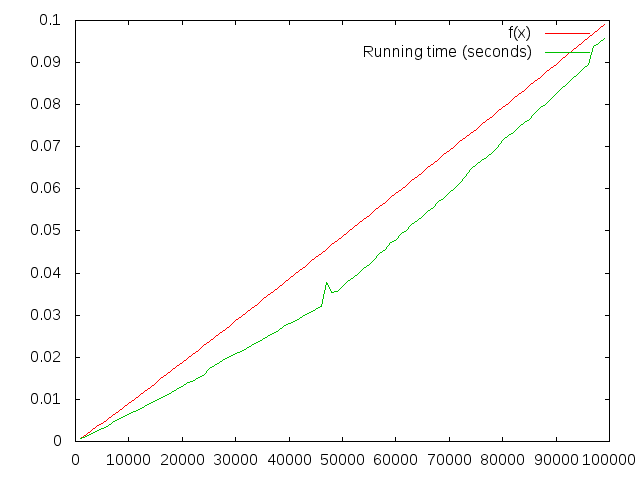
\includegraphics[scale=0.5]{erat3.png}
	\end{figure}
	
	It is evident from figure \ref{runtime1} that the function derived from the running time analysis bounds the experimental running time. So, we have a proven, efficient method for generating prime numbers up to some value.
	
	\section{Improvements and a New Sieve}
	
	Here we will begin discussing improvements to the sieve algorithm, and derive a different way to obtain prime numbers. The sieve of Sundaram operates on similar principles as the sieve of Eratosthenes, but has some differences that make it noteworthy when discussing prime generation.
	
	The sieve of Sundaram begins with a similar idea to the previous algorithm; we want to ``mark" or otherwise collect composite numbers, that are multiples of prime numbers. However, we can take advantage of an interesting result presented in lemma \ref{ijstuff} with regards to odd composite numbers.
	Once the algorithm has been presented, its asymptotic running time can be proved. We also demonstrate a plot of running time against output size, as we did with the sieve of Eratosthenes.
	
	\subsection{How to Find Odd Composites}
	
	Odd numbers can easily be written as $2k+1$ for some integer $k$. When we are trying to sieve primes, we would like to exclude those odd natural numbers that are composite; that is to say, those numbers that have a nontrivial factor. If we have some odd integer $a\geq3$, we can determine under what conditions $a$ is composite or prime.
	
	\begin{lem}\label{ijstuff}
		Let $a\geq3$ be an integer. Then $a$ can be written as $a = 2k+1$ where $k$ is of the form $k=i+j+2ij$, if and only if $a$ is a composite number.
	\end{lem}
	\begin{proof}
		We can write $a$ as
		$$ 2k + 1 = 2(i+j+2ij) + 1 . $$
		Then we can simplify to obtain
		\begin{equation*}
		\begin{split}
		a &= 2(i+j+2ij) + 1 \\
		  &= 4ij + 2j + 2i + 1 \\
		  &= 2j(2i+1) + 2i + 1 \\
		  &= (2j+1)(2i+1)
		\end{split}
		\end{equation*}
		So $a$ is an odd composite, since it has nontrivial odd factors $2j+1$ and $2i+1$.
	\end{proof}

	This result gives precisely the odd numbers where we can find primes. Now we can modify the sieve to cross out integers of the form $i+j+2ij$ up to $n$, and then obtain primes as those $2k+1$ for $3 \leq k \leq n$ that have not been crossed out.
	
	\subsection{The Sieve of Sundaram}
	
	This result was shown by an Indian mathematician, S. P. Sundaram in 1934. Unfortunately, little is known about this man, besides his invention of this sieve. 
	
	Applying lemma \ref{ijstuff}, we can write a new algorithm.

	\begin{figure}[H]\caption{Sieve of Sundaram}
		\begin{lstlisting}[language=Python]
		from math import ceil
		
		def Sundaram(n):
		    interesting_nums = set()
		    bound = int(ceil((n-2)/2))
		    for i in range(1, bound):
		        for j in range(i, int(ceil((n-i)/(1+2*i)))):
		            interesting_nums.add(2*i*j+i+j)
		
		return [2*a+1 for a in range(1,bound) if a not in interesting_nums]
		
		\end{lstlisting}
	\end{figure}

	Again, we use the set structure because of its efficiency in membership checking. This time, we use nested loops for $i$ and $j$. The proof of correctness follows easily from lemma \ref{ijstuff}.
	
	\begin{thm}
		The algorithm \texttt{Sundaram} produces the prime numbers in the range $[3, n]$.
	\end{thm}
	\begin{proof}
		The final output contains only those integers between $3$ and $n$ which are not of the form $2ij+i+j$, as these have been culled into \texttt{interesting\_nums}. We know from lemma \ref{ijstuff} that for some $a=2k+1$, if $k$ is not of the form $2ij+i+j$, $a$ is prime. So, the final output contains all such $2k+1$ for $k$ not of the form $2ij+i+j$. The algorithm has total correctness as its loop bounds are finite.
	\end{proof}
	
	\begin{thm}
		The algorithm \texttt{Sundaram} has an asymptotic running time of $O(n^2)$.
	\end{thm}
	\begin{proof}
		Once again, we will count the number of set update operations performed. We have
		\begin{equation*}
		\begin{split}
		\sum_{i=1}^{\ceil*{\frac{n-2}{2}}} \sum_{j=i}^{\ceil*{\frac{n-i}{1+2i}}} 1 & = \sum_{i=1}^{\ceil*{\frac{n-2}{2}}} \ceil*{\frac{n-i}{1+2i}} - i + 1 \\
		& = \sum_{i=1}^{\ceil*{\frac{n-2}{2}}} \ceil*{\frac{n-i}{1+2i}} - \frac{1}{8}(n^2-2n) + \ceil*{\frac{n-2}{2}}
		\end{split}
		\end{equation*}
		If we ignore the first term, we can see that the remaining terms are on the order of $n^2$. The first term is a difficult summation to solve, so instead we will create an upper bound on the summand. Because the upper bound of the summation is linear in $n$, we expect a result of $O(n^2)$.
		\begin{equation*}
		\begin{split}
		\frac{n-i}{1+2i} < \frac{n-i}{2i} < \frac{n-i}{i} & = \frac{n}{i} - 1 < \frac{n}{i} < n
		\end{split}
		\end{equation*}
		If we use $n$ to replace $\ceil*{\frac{n-i}{1+2i}}$ in the above summation, we obtain
		$$\frac{1}{2}(n^2 - 2n)$$
		and so the resulting function of the runtime analysis is $O(n^2)$.
	\end{proof}
	
	Again, we can construct a time experiment to observe the running time in practice. The results are shown in figure \ref{runtime2}. On first glance, the plot appears linear, but upon careful consideration, quadratic curvature can be observed. Note also that the sieve of Sundaram appears slower than the sieve of Eratosthenes by a factor of about two on an output size of 100000.
	
	\begin{figure}\caption{Asymptotic Running Time of \texttt{Sundaram}}
		\label{runtime2}
		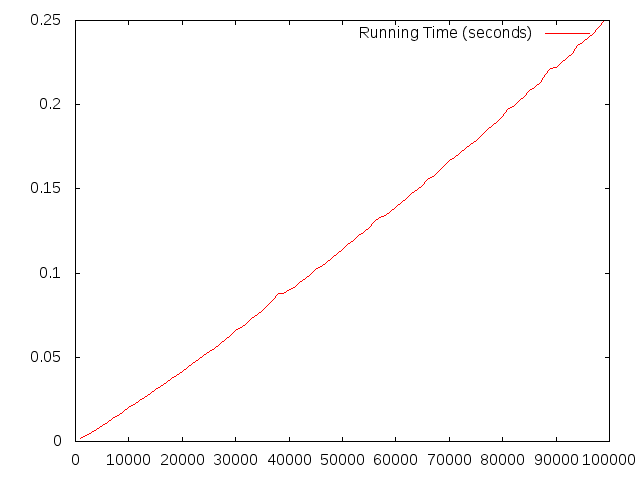
\includegraphics[scale=0.5]{sund2.png}
	\end{figure}
	
	\section{Comparison of the Two Sieves}
	
	This section will describe the two sieve algorithms we have seen and compare running time in theory and practice. We will elaborate on the details of each algorithm's shortcomings and strengths, with an interest in moving towards developing a more efficient sieve for large numbers.
	
	\subsection{Time Complexity and Practical Running Time}
	The first point to make is a comparison of the mathematically derived asymptotic running time for each sieve. While Sundaram is polynomial, Eratosthenes beats it by having a time complexity between linear and polynomial time. A comparison of theoretical running times shows that Eratosthenes is a clear winner.
	
	Noting that practical considerations are also of importance, we can test the running time as a function of output size, running each algorithm several times and taking an average. The result of a side-by-side time trial gives the plot shown in figure \ref{runtimevs}.
	
	\begin{figure}\caption{Comparison of Running Times of Both Sieves}
		\label{runtimevs}
		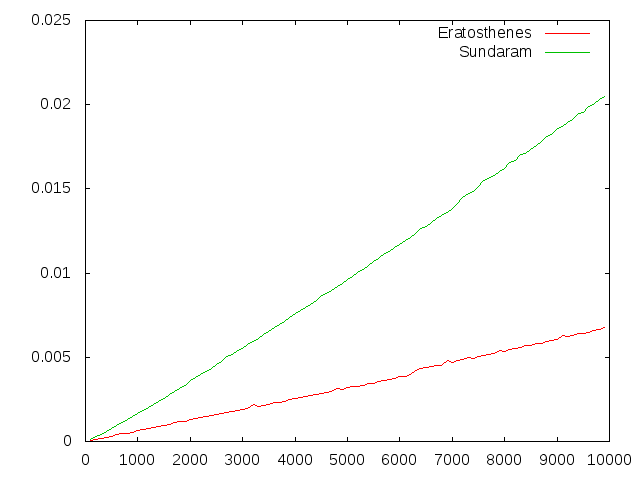
\includegraphics[scale=0.5]{both1.png}
	\end{figure}
	
	So, even when sieving smaller primes, Eratosthenes wins. Sundaram's algorithm makes clever use of lemma \ref{ijstuff}, but is still computationally inferior to Eratosthenes.

	

























\end{document}